%%
%% This is file `sample-xelatex.tex',
%% generated with the docstrip utility.
%%
%% The original source files were:
%%
%% samples.dtx  (with options: `sigconf')
%% 
%% IMPORTANT NOTICE:
%% 
%% For the copyright see the source file.
%% 
%% Any modified versions of this file must be renamed
%% with new filenames distinct from sample-xelatex.tex.
%% 
%% For distribution of the original source see the terms
%% for copying and modification in the file samples.dtx.
%% 
%% This generated file may be distributed as long as the
%% original source files, as listed above, are part of the
%% same distribution. (The sources need not necessarily be
%% in the same archive or directory.)
%%

\documentclass[sigconf, nonacm]{acmart}

\usepackage{mwe}
\usepackage[colorinlistoftodos,prependcaption,textsize=tiny]{todonotes}


%%
%% \BibTeX command to typeset BibTeX logo in the docs
\AtBeginDocument{%
  \providecommand\BibTeX{{%
    \normalfont B\kern-0.5em{\scshape i\kern-0.25em b}\kern-0.8em\TeX}}}

\begin{document}

%%
%% The "title" command has an optional parameter,
%% allowing the author to define a "short title" to be used in page headers.
\title{Express Data Queueing}

%%
%% The "author" command and its associated commands are used to define
%% the authors and their affiliations.
%% Of note is the shared affiliation of the first two authors, and the
%% "authornote" and "authornotemark" commands
%% used to denote shared contribution to the research.
\author{Freysteinn Alfreðsson}
\email{freysteinn.alfredsson@kau.se}
\orcid{0000-0003-1516-9370}
\affiliation{%
  \institution{Department of Computer Science}
  \city{Karlstad}
  \country{Sweden}
}
\author{Per Hurtig}
\email{per.hurtig@kau.se}
\affiliation{%
  \institution{Department of Computer Science}
  \city{Karlstad}
  \country{Sweden}
}
%%\orcid{0000-0003-1516-9370}
\author{Anna Brunstrom}
\email{anna.brunstrom@kau.se}
\affiliation{%
  \institution{Department of Computer Science}
  \city{Karlstad}
  \country{Sweden}
}

\author{Toke Høiland-Jørgensen}
\email{toke@redhat.com}
\affiliation{%
  \institution{Red hat}
  \country{Denmark}
}

\author{Jesper Dangaard Brouer}
\email{brouer@redhat.com}
\affiliation{%
  \institution{Red hat}
  \country{Denmark}
}

%%
%% By default, the full list of authors will be used in the page
%% headers. Often, this list is too long, and will overlap
%% other information printed in the page headers. This command allows
%% the author to define a more concise list
%% of authors' names for this purpose.
\renewcommand{\shortauthors}{Alfreðsson, et al.}

\begin{abstract}
\end{abstract}

%%
%% Keywords. The author(s) should pick words that accurately describe
%% the work being presented. Separate the keywords with commas.
\keywords{XDP, BPF, BPF, Queueing, Linux, Scheduling}

%%
%% This command processes the author and affiliation and title
%% information and builds the first part of the formatted document.
\maketitle

\section{Introduction}

The Linux kernel is a widely used platform in devices that range from IoT devices, cellphones, home and enterprise routers to servers and cloud offerings. One of the revolutionary technologies of the Linux kernel is the BPF framework, which has changed the way we extend the kernel. This framework is an in-kernel runtime environment that allows domain-specific code to execute within the kernel safely using predefined hooks. One such hook is the Linux eXpress Data Path\cite{hoiland2018express}, or XDP, which has found numerous uses in the industry, such as DoS attack mitigation, load-balancers, and intrusion prevention systems.

XDP provides a high-performance programmable network data path and allows programmers to process packets early out of the driver. While XDP excels in forwarding packets, it currently has no mechanism for queuing or reordering of packets and cannot implement traffic scheduling policies. Packet scheduling is a common task on network equipment, and like for other aspects of networking, there is a growing interest for bringing programmability to this domain. For the Linux kernel, making packet scheduling fully programmable through BPF is the obvious answer to this trend.

This paper presents our work on adding programmable packet scheduling to XDP, which we also provide as a Qdisc. We have designed a programmable packet scheduling framework in BPF using recently proposed schemes for programmable queues. This extension allows programmers to define their packet schedulers using BPF while benefiting from the XDP fast data path.


\begin{itemize}
\item Explain the structure of this technical report.
\end{itemize}

\section{Packet Scheduling, Traffic Shaping, and Queue Management}

The primary function of the packet scheduler is to arrange or rearrange packets to meet some specific requirements within its network. Most of these requirements is to prioritize one type of traffic over another. For instance, a video streaming services would like to ensure that clients get fair access to their video streams. And a service provider might want to prioritize the traffic of their productions servers over their testing servers.

Another important component related to packet schedulers is the capability of delaying packets. This capability allows packet scheduling algorithms to provide traffic shaping or pacing.  service from using all of the traffic, or it could make sure that important traffic never gets delayed.

Queue management, on the otherhand, is how many packets the queues are able to queue up. A large problem in today's environments is buffer bloat, where buffers tend to favor large buffers for throughput with the cost of latency. Buffer bloat can have negative affects on low latency applications such as video conferecing, on-line gaming, and other interactive applications. Queue management is therefore an important part of the queueing process, while it is not usually concidered part of the packet scheudling algorithms.

\begin{itemize}
  \item Explain the difference between a work-conserving and non-work conserving scheduling.
  \item Use a short round-robin scheduling example.
\end{itemize}


\section{Linux Kernel Networking Subsystem}

\begin{figure}

  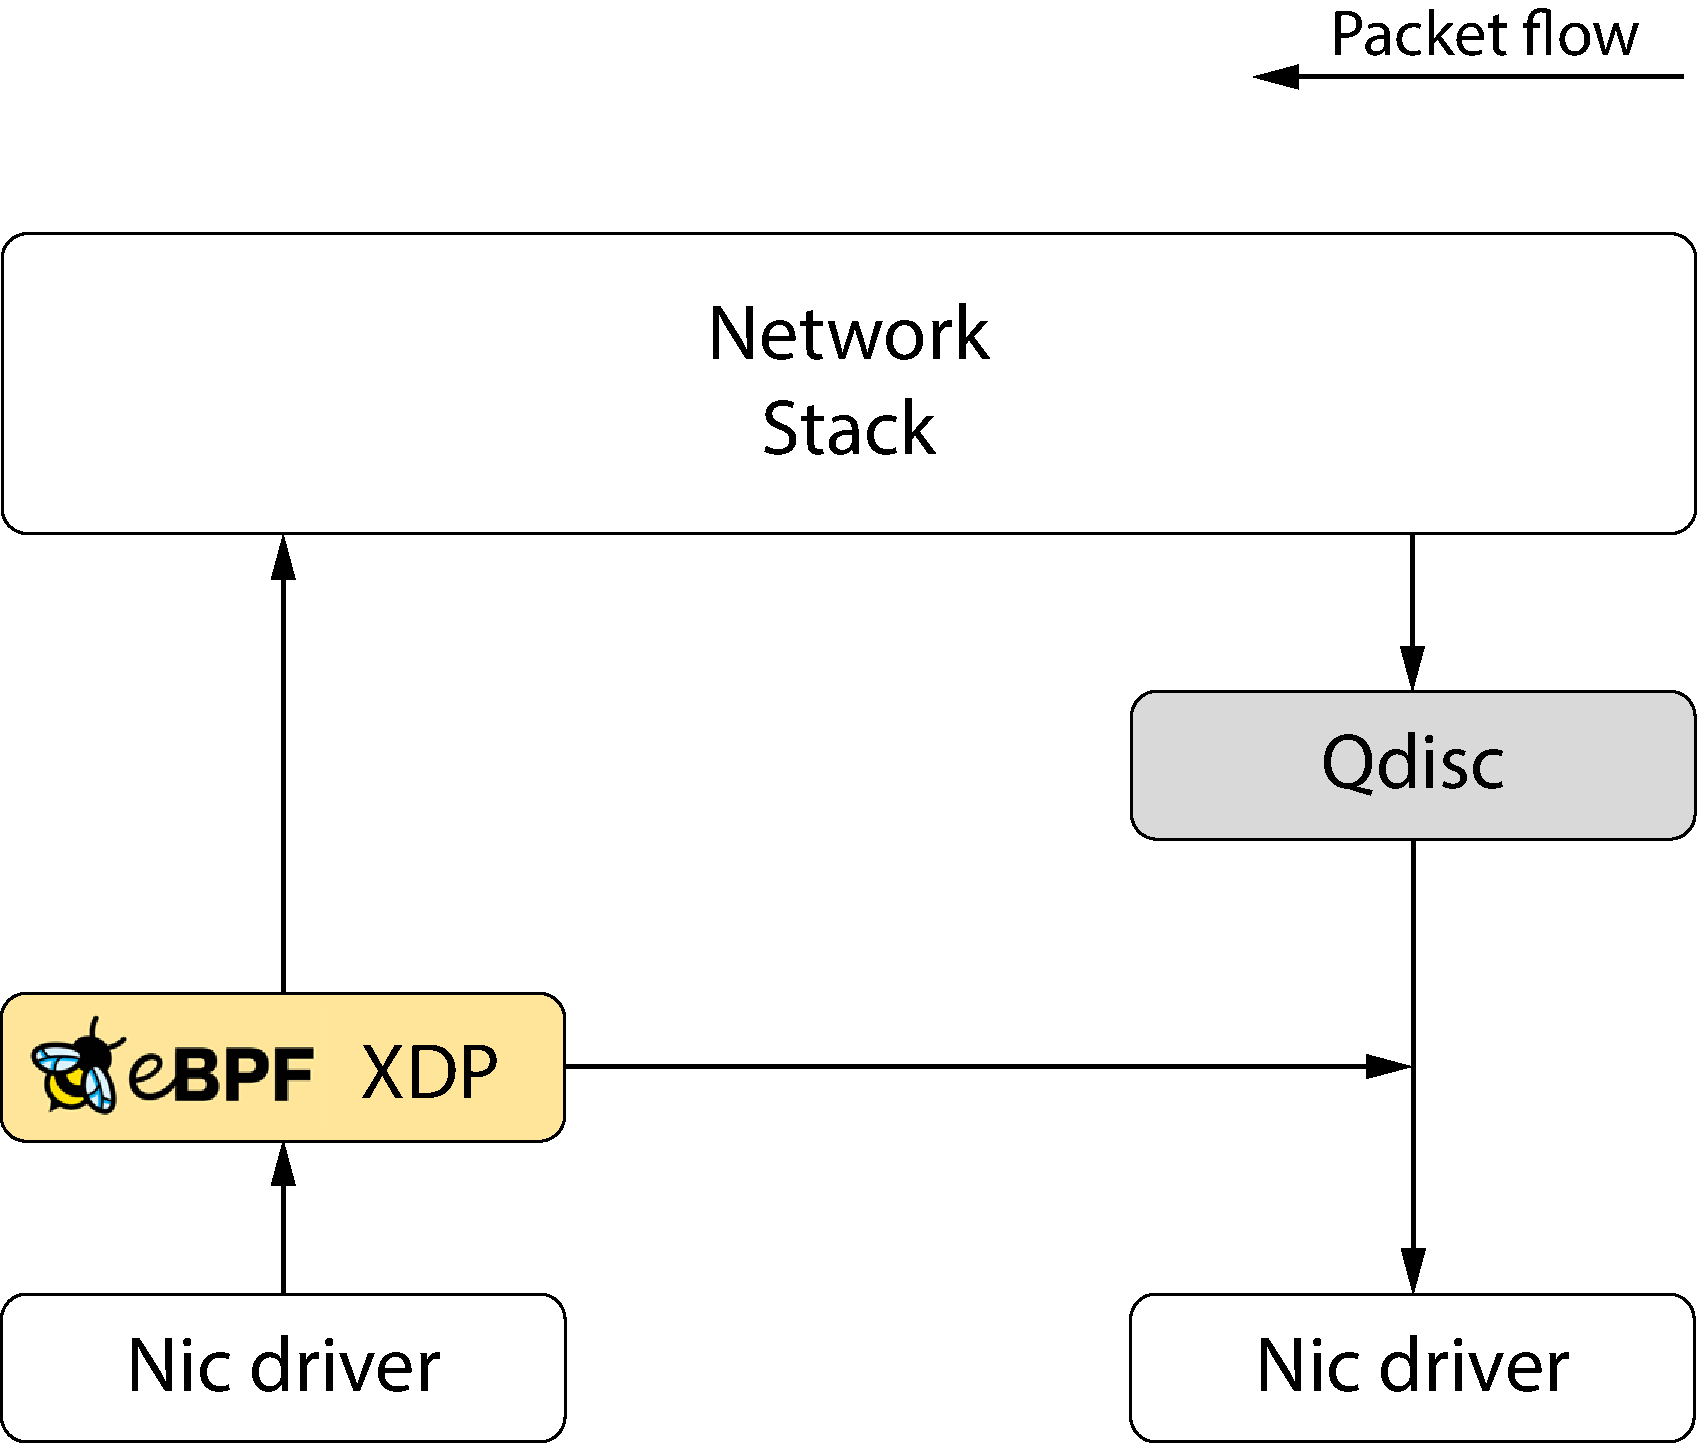
\includegraphics[width=\linewidth]{network-overview.pdf}

  \caption{\label{fig:network_overview}}
\end{figure}

\begin{itemize}
  \item Explain on a high level the Linux Kernel Networking stack using a diagram.
\end{itemize}

\subsection{The Linux Kernel Packet Queueing Discipline (Qdisc)}

\begin{itemize}
  \item Explain where in the network pipe the Qdiscs are located.
  \item Explain, without going into too much detail, what the Qdisc system is capable of.
        \begin{itemize}
          \item Shaping: Shaping delay packets to meet a desired rate.
          \item Scheduling: Schedulers arrange and/or rearrange packets for output.
          \item Classifying: Classifiers sort or separate traffic into queues.
          \item Policing: Policiers measure and limit traffic in a particular queue.
          \item Dropping: Dropping discards an entire packet, flow or classification.
          \item Marking: Marking is a mechanism by which the packet is altered.
        \end{itemize}
  \item Explain what type of primitives the Qdiscs system supplies:
        \begin{itemize}
          \item Classfull Qdiscs.
          \item Classless Qdiscs.
          \item Filters.
        \end{itemize}
\end{itemize}


\section{Packet Schedulers in Practice}

\todo[inline]{Frey: This section needs a new name. The idea with this section is to explain why we care about this work and what the requirements are.}

\begin{itemize}
  \item Explain what is not possible using today's packet schedulers.
  \item Explain why you would like to be able to schedule traffic
\end{itemize}


\section{Programmable Packet Schedulers}

\todo[inline]{Frey: Maybe this section could be combined with the above section if we find a better name for them.}

\begin{itemize}
  \item Explain how programmable packet schedulers differ from traditional schedulers.
  \item Explain what we want from a programmable packet scheduler.
        \begin{itemize}
          \item Can handle work and non-work conserving scheduling.
          \item Can combine data structures to form a hierarchy for more advanced algorithms.
        \end{itemize}
\end{itemize}

\todo[inline]{Frey: In the original draft I had a special section called algorithm for each of the data structures below. I decided to remove it for now because I think it is intertwined with the data structure.}


\subsection{PIFO and SP-PIFO}

\begin{itemize}
  \item Explain what PIFO\cite{Sivaraman2016} is.
  \item Explain how PIFO does not allow scheduling at dequeue, but can form hierarchies to create more complex logic.
  \item Explain that SP-PIFO\cite{Alcoz2020} approximates the behavior of a PIFO using Strict-Priority queues.
  \item Explain that does not support non-work conserving scheduling.
\end{itemize}


\subsubsection{Data Structure}

\begin{itemize}
  \item Explain how the PIFO is an array of queues.
  \item Explain how the PIFO tends to not scale with large sizes. Mainly in hardware based scheduling.
  \item Explain how the SP-PIFO is a small PIFO that approximates larger PIFO.
\end{itemize}


\subsection{Eiffel}

\begin{itemize}
  \item Explain how Eiffel\cite{Saeed2019} data structure is designed for software based scheduling and that it is optimized using find-first-set instructions.
  \item Explain that it can change the order of the packets on dequeue, unlike PIFO.
\end{itemize}


\subsubsection{Data Structure}

\begin{itemize}
  \item Explain that it uses a bitmap to keep track of available slots for optimization with FFS commands.
  \item Explain that it uses two alternating data structures to allow incremental inserts while not needing to scale the bitmaps dynamically.
\end{itemize}


\subsection{Calendar-queues}

\begin{itemize}
  \item Explain that it supports both work and non-work conserving scheduling.
\end{itemize}


\subsubsection{Data Structure}

\begin{itemize}
  \item Explain that it uses a circular buffer with a hand like an analog clock. The slots represent when the scheduler will dequeue in the future. While the hand points to the packets that are dequeing.
\end{itemize}


\section{The BPF framework}

The BPF framework is an in-kernel runtime environment that allows specialized
programs to execute in the kernel safely. These programs attach themselves to
hooks provided by the different subsystems of the kernel. These hooks limit what
the programs can do and define what type of BPF programs can exist. These types
of programs vary but predominantly, they are related to networking, tracing, and
security. At its core, BPF is an instruction set. However, as a framework, it
provides a key-value store that enables inter-process communication called BPF
maps, in-kernel helper functions, and toolchains to create and manage BPF
programs from user-space.

\todo[inline]{Frey: Because we all know what BPF is, I am going to collapse these BPF sections and make it shorter and simpler.}

\begin{itemize}
  \item Explain h
  \item Explain BPF maps and their scope.
  \item Explain what hooks are and that BPF allows helper functions.
  \item Explain how BPF programs are loaded using the bpf system call.
\end{itemize}


\subsection{Instruction-set}

\todo[inline]{Frey: I think I will remove this section either completely, or at least remove the extra details.}

The BPF instruction set is 64-bit and consists of eleven registers listed in
table ~\ref{table:BPF_registers}. It contains a little over a hundred
instructions. However, the current format defines the opcode as the first octet
of the instruction. Therefore, in the current design, it could only support 256
instructions. The currently available instructions are limited to Arithmetic
Logic Unit (ALU) instructions, byte-swap instructions for Endian handling,
memory, and branch instructions.

\begin{table}
  \caption{Frequency of Special Characters}
  \label{table:BPF_registers}
  \begin{tabular}{ll}
    \toprule
    Register & Type                    \\
    \midrule
    R0       & Return value            \\
    R1-R5    & Parameters to functions \\
    R6-R9    & Callee saved registers  \\
    R10      & Read-only stack pointer \\
    \bottomrule
\end{tabular}
\end{table}


\subsection{Express Data Path (XDP)}

XDP\cite{hoiland2018express} is a type of BPF program that is attached directly to the RX path of a network interface to allow the programmer direct manipulation of packets from the network driver. Its primary use cases are high-performance packet processing and the ability to bypass the kernel's network stack by redirecting the packet to different locations, such as back out the same device, to another device, or dropping the packet entirely. XDP also provides helper functions that allow the programmer to call particular parts of the network stack, such as fib lookups.

While XDP excels at forwarding packets, it does not support packet reordering or packet scheduling. Our objective in this paper is to extend XDP to support packet scheduling. This support includes adding helper functions and extra hooks for dequeuing and pacing operations.


\subsection{BPF Qdisc Classifiers}

Currently, the Qdisc layer only has a BPF classifier capable of manipulating packets and directing them into excising Qdiscs that are not programmable using BPF. While this does provide a form of programable packet scheduling, it relies exclusively on the Qdisc layer, which XDP can not use. We aim to provide a BPF based packet scheduling framework for XDP and as a standalone Qdisc.


\section{A Programmable Packet Scheduling Framework in BPF}

\begin{figure}

  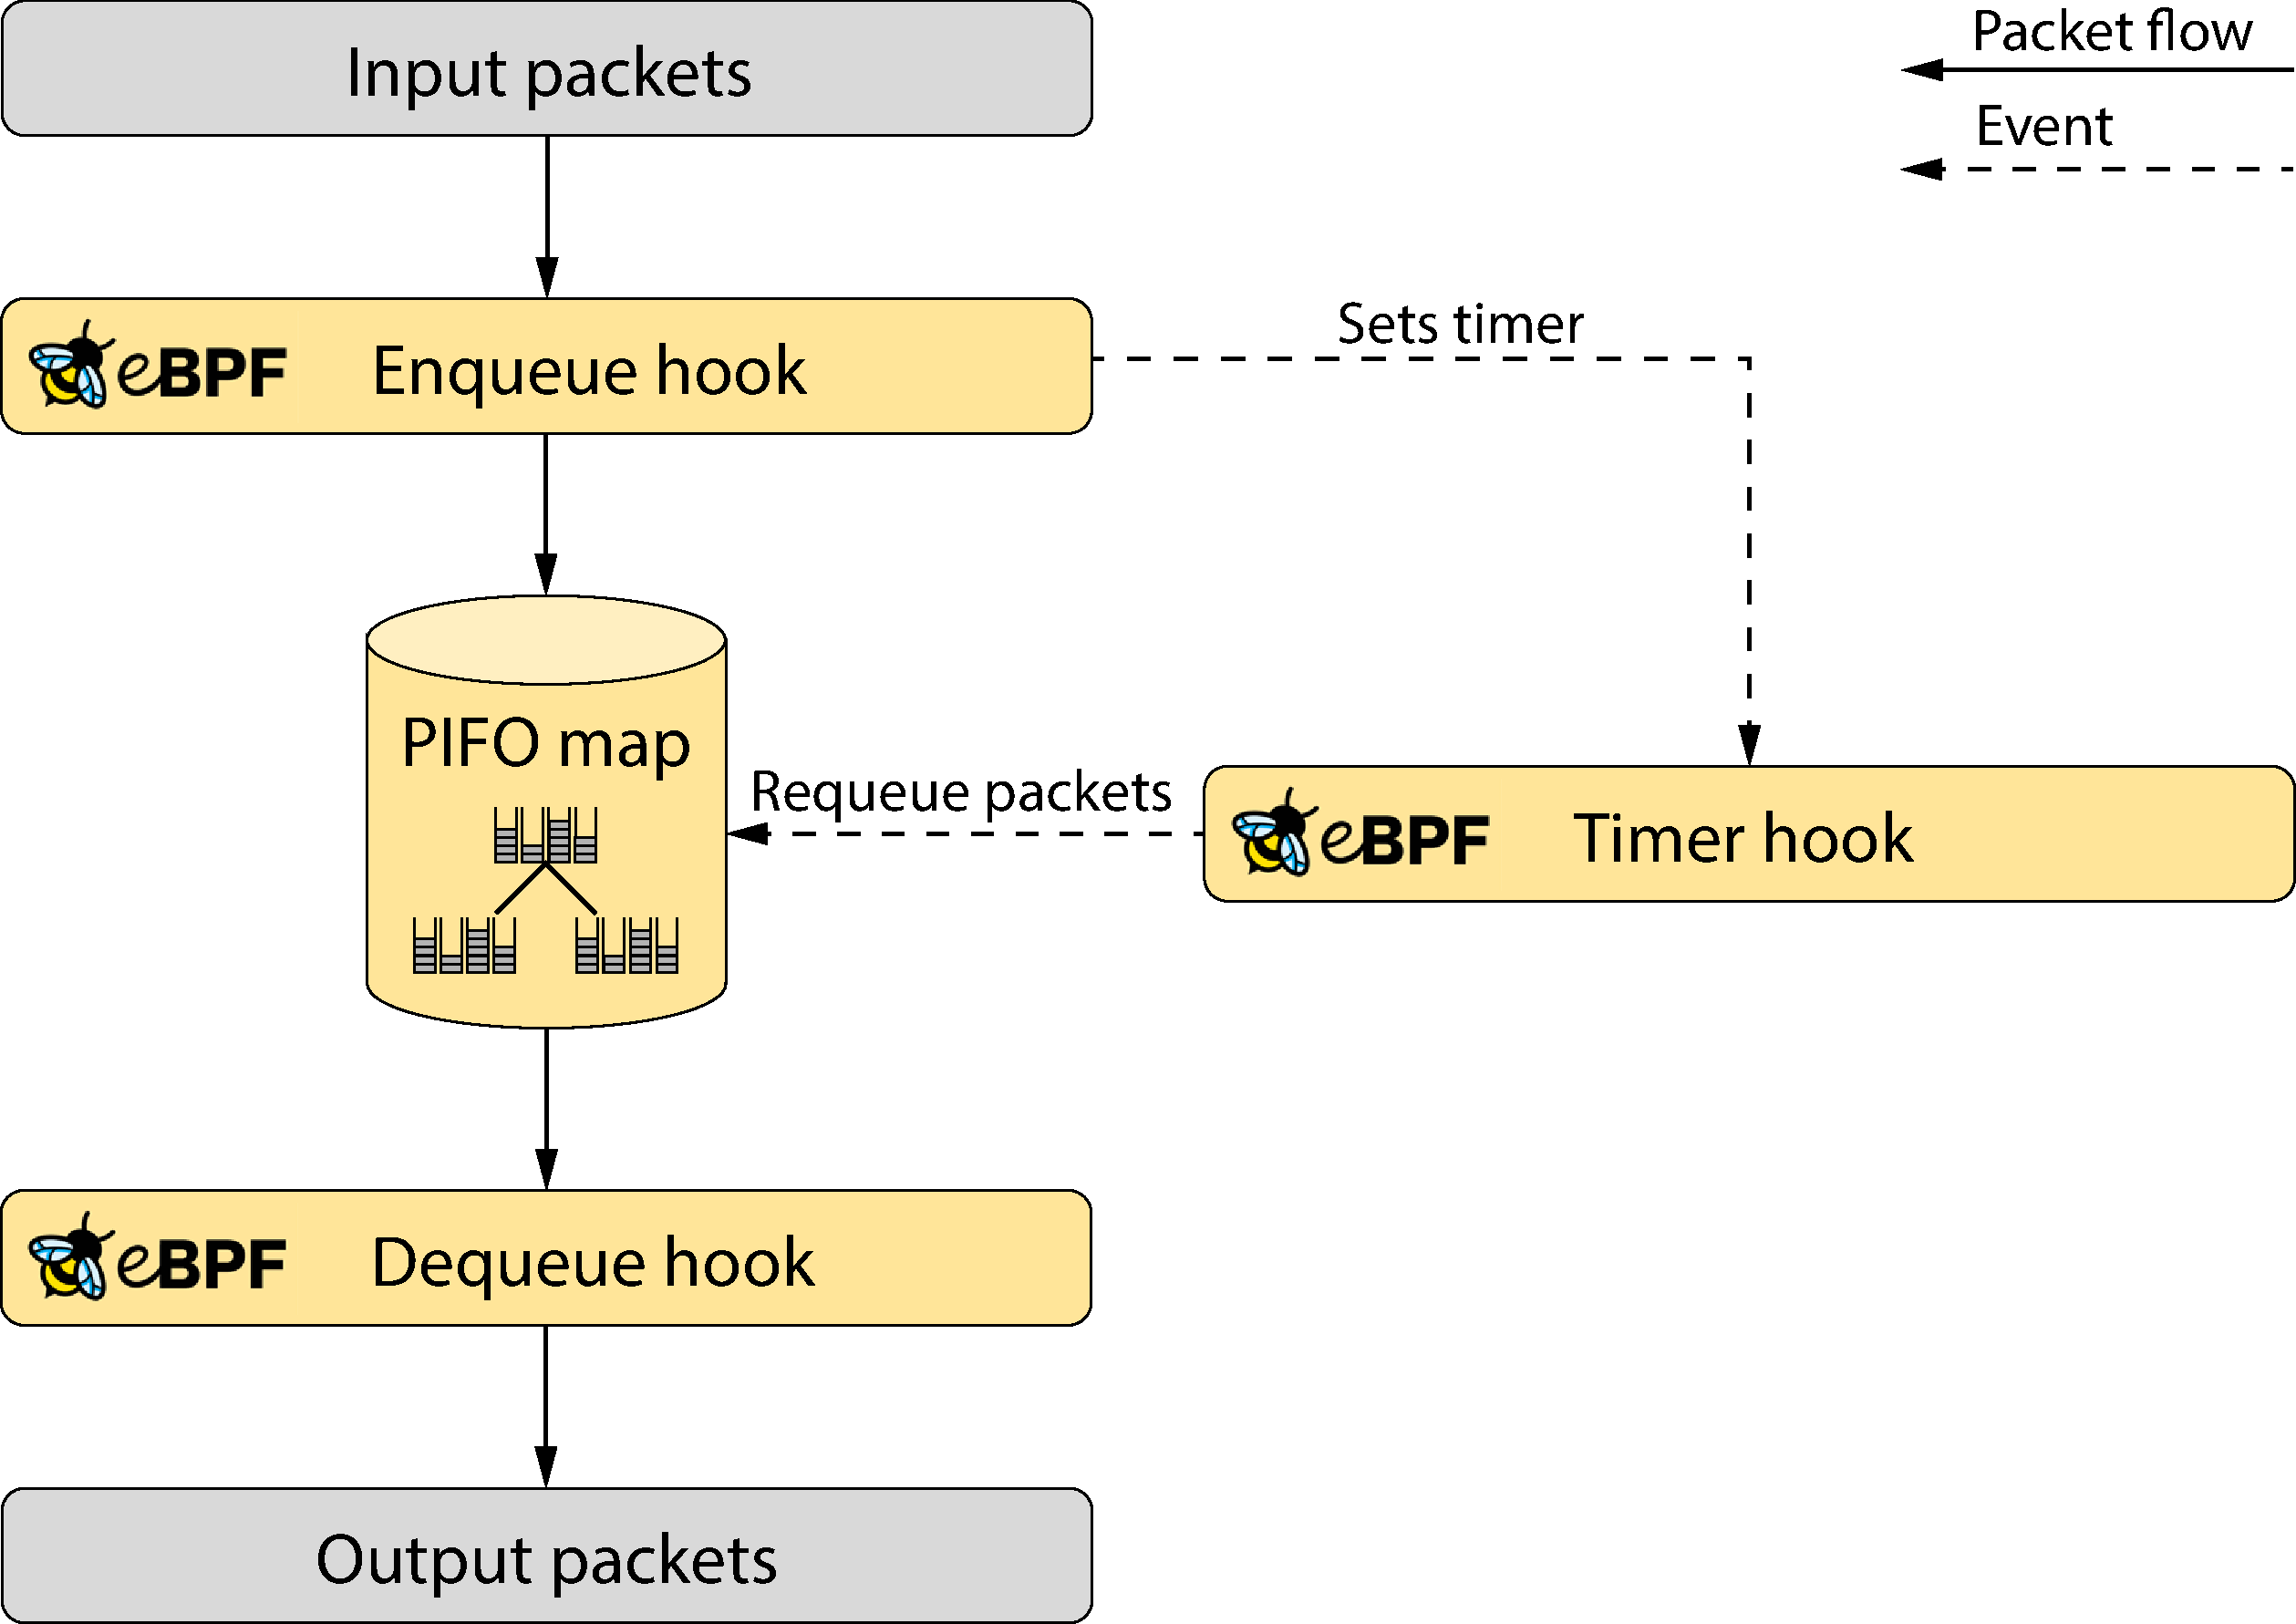
\includegraphics[width=\linewidth]{bpf_pps_flow.pdf}

  \caption{Depicted are the BPF hooks needed to implement programmable packet scheduling using our new proposed framework. The main hooks are the enqueue and dequeue hooks, with the optional timer hook. Queueing works the same in both XDP and the Qdisc. However, they do not use the same enqueue and dequeue hooks.\label{fig:bpf_pps_flow}}

\end{figure}

Our vision is to create an BPF based programmable packet scheduling framework that is flexible enough to share between the XDP and kernel Qdisc layers. The design is depicted in Figure \ref{fig:bpf_pps_flow}, which shows the basic building blocks for our design without the specifics of XDP nor the Qdisc subsystem.

These building blocks are then further broken down as follows:

\begin{itemize}
        \item Queue map: This new BPF map implements a PIFO and is the main building block for the programmer to create packet schedulers.
        \item Enqueue hook: This BPF hook is responsible for redirecting packets to BPF queue maps. This is the standard XDP hook in the case of XDP. However, it is a new hook in Qdiscs.
        \item Timer hook: This is an optional hook and is only required for algorithms that delay packets, e.g., packet pacing or traffic shaping. It is responsible for dequeuing and enqueuing packets from different PIFOs to introduce delayed packets. We implement timers using the newly introduced BPF timer API. This API allows the programmer to schedule BPF programs to be run at a specified time in the future, which can be used to release held packets.
        \item Dequeue hook: This hook is responsible for delivering the packet from the packet scheduling algorithm. In XDP, this is a new hook that each driver calls to transmit a packet. It can deliver bulking by repeatedly calling the hook to dequeue multiple packets before it transmits them.
\end{itemize}

Our design represents the PIFO data structure as an eBPF map. This representation allows the BPF programs to use a familiar map interface to reference PIFOs straightforwardly in their scheduling algorithm. From a programmer's perspective, the eBPF hooks reference the queues like any other map type. The enqueue hook can decide which queue to direct the packet to by a map reference. Similarly, the dequeue hook can pick which queue map to dequeue from and return a reference to the dequeued packet to the kernel for transmission. The BPF packet scheduling hooks can set BPF timers that trigger BPF programs at specified times if the scheduling algorithm needs to implement shaping and pacing. The BPF timer API supports both microsecond and nanosecond precision using the kernel's \textit{hrtimers}, making it ideal for our use case.


\section{BPF-Qdisc}

Due to XDP being only available in ingress and not at egress, queuing is only suitable for forwarded packets. However, if we want to support packets from the local machine, we provide a BPF-Qdisc that supports XDQ the same way as in XDP. To support this, we have created a new Qdisc that includes two separate hooks for ingress and egress to reflect our original design.


\section{eXpress Data Queueing (XDQ)}

Our design extends XDP by adding a new dequeue hook into the network drivers. We
rely on standard XDP to enqueue packets into BPF queue maps. However, the new
dequeue hook supports bulking by having the driver repeatedly dequeue packets
from the dequeue hook before it transmits the packets.


\section{Evaluation of BPF-Qdisc and XDQ}

\begin{itemize}
  \item Compare a type of scheduling algorithm using BPF-Qdisc and XDQ performance to Qdiscs that does the same functionality.
  \item Compare BPF-Qdisc and XDQ performance to eachother.
\end{itemize}

\section{Conclusion}

\begin{itemize}
  \item Reiterate main points of design, and summarize results.
\end{itemize}



\bibliographystyle{ACM-Reference-Format}
\bibliography{references}


\end{document}
\endinput
